\section{Experiments}
\label{sec:experiments}

\subsection{Experiment Setup}
\label{sec:setup}

\paragraph{Models.}
Following prior work on multi-turn on-policy distillation, we use teacher and student models from the same model family to reduce confounding effects from tokenizer, architecture, and instruction-format mismatch. Specifically, we use Qwen3-32B and Qwen3-8B as teacher models, and Qwen3-0.6B and Qwen3-1.7B as student models \citep{yang2025qwen3}. This yields multiple teacher--student pairs with different capacity gaps, allowing us to evaluate whether \ours{} remains effective across both large-gap and moderate-gap distillation settings.

\paragraph{Datasets and Evaluation.}
We evaluate \ours{} on three multi-turn agent benchmarks: ALFWorld \citep{shridhar2020alfworld}, ScienceWorld \citep{wang2022scienceworld}, and SearchQA \citep{jin2025search}. These benchmarks cover embodied interaction, scientific task solving, and search-based question answering, respectively, allowing us to assess the effectiveness of selective intervention across different forms of multi-turn decision making.

For ALFWorld, we report success rate (SR) on both the seen and unseen splits. For ScienceWorld, we report success rate (SR) and the mean score on the test set. For SearchQA, we report exact match (EM) across different question-answering datasets. Detailed definitions of the evaluation metrics are provided in \appref{sec:implementation_details}.

\paragraph{Baselines.}
We compare \ours{} with four main baselines: off-policy SFT, vanilla OPD, TCOD (F2B) \citep{wang2026tcod}, and Entropy-Aware OPD \citep{jin2026entropy}. TCOD-F2B stabilizes multi-turn OPD through a forward-to-backward temporal curriculum, and Entropy-Aware OPD augments OPD with entropy-gated KL loss originally designed for single-turn distillation. 
%
Since \ours{} uses one additional teacher query to obtain the turn-level intervention label, it introduces extra inference cost compared with vanilla OPD.
%
In practice, this overhead is limited because most prompt tokens are shared with the rollout context and can be cached, while the intervention output is only a short label.
%
Nevertheless, to control for the additional teacher-query budget, we include a compute-matched baseline, vanilla OPD with two rollouts, where both the student and teacher are queried twice during OPD data collection.

\paragraph{Training Details.}
We implement OPD with a fully asynchronous rollouter--trainer pipeline. Unless otherwise specified, all methods are trained for one epoch with learning rate $1\times10^{-6}$ and rollout number 1. We use student temperature $0.4$, teacher temperature $0.0$, top-$p=1.0$, and top-$k=-1$ as the default setup. For \ours{}, we set the weak-intervention coefficient to $\alpha=0.5$. We analyze the sensitivity to this choice in \secref{sec:sensitivity_analysis}. Additional implementation details are provided in \appref{sec:implementation_details}.


\subsection{Main Results}
\label{sec:result_analysis}

\begin{table*}[t]
\centering
\caption{Main results on ALFWorld. We report success rate (SR) and average number of turns on both seen and unseen splits. Best SR among distillation methods for each student--teacher setup is in \textbf{bold}, and the second-best SR is \underline{underlined}.}
\label{tab:main_results_alfworld}
\resizebox{0.95\textwidth}{!}{%
\begin{tabular}{lllcccc}
\toprule
\textbf{Student Model} & \textbf{Teacher Model} & \textbf{Method}
& \textbf{Seen SR} & \textbf{Seen Turns}
& \textbf{Unseen SR} & \textbf{Unseen Turns} \\
\midrule
\multicolumn{7}{c}{\textit{Reference Models (Base Inference)}} \\
\midrule
Qwen3-0.6B & -- & Base & 1.43 & 29.65 & 0.75 & 29.82 \\
Qwen3-1.7B & -- & Base & 25.71 & 24.63 & 26.12 & 24.72 \\
-- & Qwen3-8B & Base & 61.43 & 17.95 & 67.16 & 17.24 \\
-- & Qwen3-32B & Base & 57.14 & 18.94 & 69.40 & 18.21 \\
\midrule
\multicolumn{7}{c}{\textit{Student: Qwen3-0.6B, Teacher: Qwen3-8B}} \\
\midrule
\multirow{6}{*}{Qwen3-0.6B} & \multirow{6}{*}{Qwen3-8B} & SFT & 2.86 & 29.32 & 4.48 & 28.87 \\
 & & OPD & 55.00 & 18.53 & 56.72 & 20.30 \\
 & & OPD (rollout 2) & \underline{56.43} & 18.76 & 59.70 & 20.31 \\
 & & Entropy-Aware OPD & 54.26 & 18.12 & 54.48 & 20.75 \\
 & & TCOD-F2B & \underline{56.43} & 18.51 & \underline{61.19} & 18.82 \\
 & & \ours{} & \textbf{57.86} & 18.46 & \textbf{61.94} & 18.89 \\
\midrule
\multicolumn{7}{c}{\textit{Student: Qwen3-1.7B, Teacher: Qwen3-8B}} \\
\midrule
\multirow{6}{*}{Qwen3-1.7B} & \multirow{6}{*}{Qwen3-8B} & SFT & 25.00 & 24.58 & 26.12 & 24.54 \\
 & & OPD & 60.00 & 17.80 & 61.94 & 17.67 \\
 & & OPD (rollout 2) & 63.00 & 17.51 & 64.93 & 17.87 \\
 & & Entropy-Aware OPD & 63.57 & 17.28 & \underline{65.67} & 18.20 \\
 & & TCOD-F2B & \textbf{64.29} & 17.65 & 58.21 & 19.16 \\
 & & \ours{} & \textbf{64.29} & 18.14 & \textbf{70.15} & 17.86 \\
\midrule
\multicolumn{7}{c}{\textit{Student: Qwen3-0.6B, Teacher: Qwen3-32B}} \\
\midrule
\multirow{5}{*}{Qwen3-0.6B} & \multirow{5}{*}{Qwen3-32B} & OPD & 53.57 & 19.49 & 68.66 & 18.65 \\
 & & OPD (rollout 2) & 52.14 & 20.28 & \underline{70.37} & 18.21 \\
 & & Entropy-Aware OPD & 48.57 & 20.87 & 68.13 & 18.28 \\
 & & TCOD-F2B & \textbf{54.29} & 20.18 & 67.91 & 19.26 \\
 & & \ours{} & \textbf{54.29} & 19.85 & \textbf{70.90} & 17.98 \\
\midrule
\multicolumn{7}{c}{\textit{Student: Qwen3-1.7B, Teacher: Qwen3-32B}} \\
\midrule
\multirow{5}{*}{Qwen3-1.7B} & \multirow{5}{*}{Qwen3-32B} & OPD & 58.57 & 18.89 & \underline{74.85} & 17.16 \\
 & & OPD (rollout 2) & \underline{62.14} & 18.17 & 72.39 & 18.37 \\
 & & Entropy-Aware OPD & 60.00 & 18.80 & \textbf{79.10} & 16.75 \\
 & & TCOD-F2B & 57.14 & 19.42 & 73.13 & 17.87 \\
 & & \ours{} & \textbf{62.82} & 18.75 & 73.88 & 17.57 \\
\bottomrule
\end{tabular}%
}
\end{table*}

We present the main results on ALFWorld, ScienceWorld, and SearchQA in \tabref{tab:main_results_alfworld}, \tabref{tab:main_results_scienceworld}, and \tabref{tab:main_results_searchqa} in \appref{sec:supplementary_results}, respectively.

\paragraph{Improvements over Base Models, SFT, and Vanilla OPD.}
Across all three benchmarks, \ours{} substantially improves over base student models and off-policy SFT. 
%
On ALFWorld, Qwen3-0.6B improves from $1.43/0.75$ SR on seen/unseen splits to $57.86/61.94$ with a Qwen3-8B teacher, while reducing the average number of turns from nearly $30$ to about $18$--$19$. 
%
Compared with vanilla OPD, \ours{} further improves Qwen3-0.6B from $55.00$ to $57.86$ seen SR and from $56.72$ to $61.94$ unseen SR, while improving Qwen3-1.7B unseen SR from $61.94$ to $70.15$. 
%
These gains are not merely due to extra teacher queries, as \ours{} also outperforms the compute-matched OPD rollout-$2$ baseline in most ALFWorld settings, with comparable or fewer turns on the unseen split.

\paragraph{Comparison with Strong OPD Variants.}
Compared with TCOD-F2B and Entropy-Aware OPD, \ours{} is strongest on ALFWorld and remains competitive on ScienceWorld and SearchQA. 
%
On ALFWorld, \ours{} achieves the best unseen SR in three out of four student--teacher settings and ties for the best seen SR in two settings, while generally maintaining similar turn efficiency to the strongest baselines. 
%
On SearchQA, \ours{} obtains the best average EM for Qwen3-1.7B distilled from Qwen3-8B, improving over OPD from $30.09$ to $30.77$. 
%
On ScienceWorld, \ours{} achieves the best SR for Qwen3-1.7B with both Qwen3-8B and Qwen3-32B teachers, and improves the Qwen3-0.6B mean score with Qwen3-8B from $-12.88$ under OPD to $+3.89$, although this comes with a higher average number of turns, suggesting more sustained task exploration.

\paragraph{Effects of Student and Teacher Scale.}
The benefits of \ours{} are more consistent for the larger Qwen3-1.7B student, which achieves strong gains on ALFWorld, the best average SearchQA result, and the best ScienceWorld SR across both teacher settings. 
%
For Qwen3-0.6B, OPD already provides large gains over SFT and base inference, while \ours{} further improves ALFWorld generalization but shows more task-dependent effects on ScienceWorld and SearchQA. 
%
Increasing teacher size is not uniformly beneficial, suggesting that stronger teacher signals are not automatically more reliable when applied densely and that adaptive weighting is important for multi-turn OPD.


\begin{figure*}[t]
    \centering
    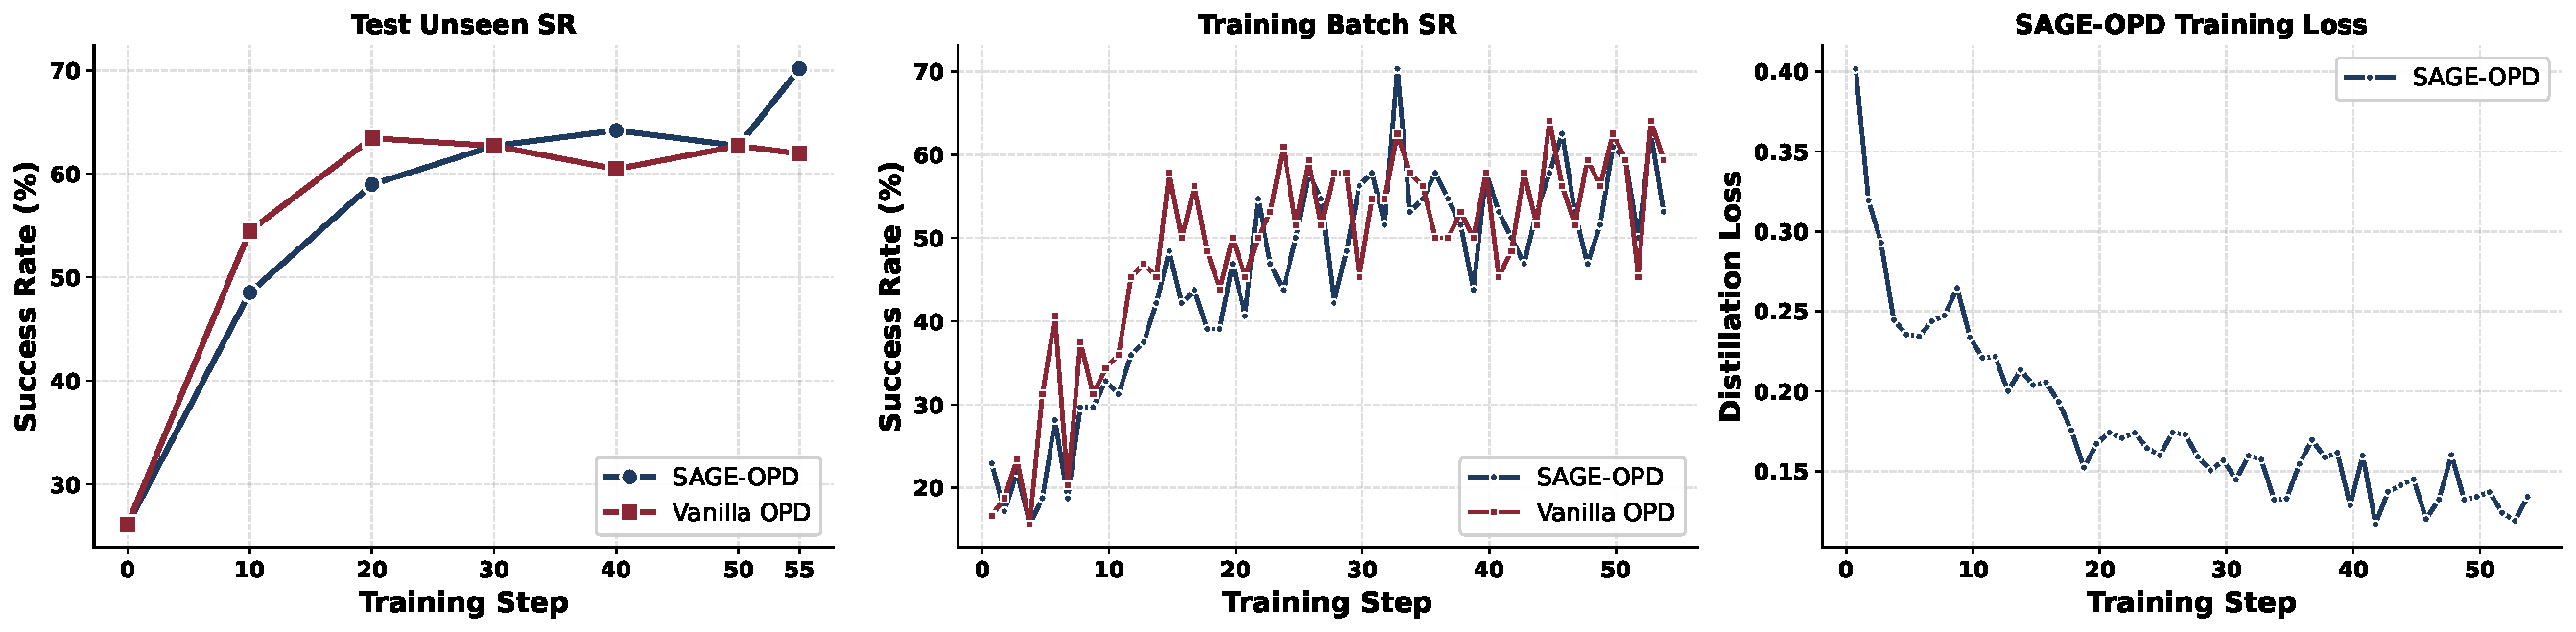
\includegraphics[width=\textwidth]{figure/alfworld_sl_opd_vs_vanilla.pdf}
    \caption{Training dynamics on ALFWorld comparing \ours{} with vanilla OPD. Left: test unseen success rate during training. Middle: training-batch success rate. Right: training loss of \ours{}.}
    \label{fig:training_dynamics}
\end{figure*}

\subsection{Training Dynamics}

\figref{fig:training_dynamics} compares the training dynamics of \ours{} and vanilla OPD on ALFWorld. 
%
On the unseen test split, both methods improve rapidly in the early stage, but vanilla OPD saturates after roughly 20--30 training steps, fluctuating around $60$--$63\%$ SR. 
%
In contrast, \ours{} continues to improve in the later stage and reaches $70.15\%$ unseen SR by the end of training. 
%
This suggests that selective intervention does not merely accelerate early learning, but also helps maintain useful teacher supervision after vanilla dense OPD begins to plateau.

The training-batch success rate shows a similar trend: both methods improve throughout training, while \ours{} remains competitive with vanilla OPD despite applying supervision selectively rather than uniformly. 
%
The right panel further shows that the \ours{} distillation loss decreases steadily over training, indicating stable optimization under the intervention-weighted objective. 
%
Together, these dynamics support our hypothesis that selectively reallocating teacher supervision can improve generalization while preserving stable on-policy training.